\subsubsection{\lephad trigger selection}
\label{sec:lephadtrigger}
In the \lephad channel, events are selected using single lepton triggers (SLT) and lepton tau triggers (LTT). 

The priority is given to SLT events if a lepton ($e$ or $\mu$) fulfils the offline lepton \pT requirements.
Single muon triggers (SMT) require an event with a muon with \pT > 21 or > 27~\GeV, whereas single electron triggers (SET)
require an event with an electron with \pT > 25 or > 27~\GeV, depending on the data-taking period.
The SLT triggers used are listed in Table \ref{tab:SLTtriggers_lephad}. 

If the event fails the SLT, then the LTT is checked. The LTT requires either an electron with \pT >18~\GeV~or a
muon with \pT > 15~\GeV. The \pT threshold for \tauhad is 30 \GeV. The complete list of LTT triggers, along with the trigger-dependent offline \pT thresholds, are
shown in Table \ref{tab:LTTtriggers_lephad}, where the abbreviations for the trigger names are used.
The full name of these triggers can be found in Table \ref{tab:LTT_trigger_names} of Appendix \ref{sec:appendix_LTT_trigger_names}.

Both for muon and electron channels, \verb|*_tau25(_EF)| triggers require one additional jet with 25 \GeV\ at L1. 
That necessitates to require one jet with offline \pT > 80 \GeV~in the analysis.

Triggers with L1 seeds \verb|*_4J12| and \verb|*_3J12|, also require additional jets at L1,
which necessitates to require two jets with offline \pT > 45 \GeV~in the analysis.

There is no jet requirement at L1 for \verb|mu14_tau35(_EF)|. 

When an OR of multiple triggers is used in the electron channel (ETT), \verb|*_4J12| trigger is prioritized due to lower jet \pT thresholds. 
This means that, other triggers are checked if and only if  \verb|*_4J12| doesn't fire. The offline selection is adjusted accordingly, as shown in Table \ref{tab:LTTtriggers_lephad}.

For 2017 and 2018 data-taking periods, different muon tau triggers (MTT)
are used for two different regions defined by 30 \GeV~< $\pT^{\tau} \leq$ 40 \GeV~ and $\pT^{\tau}$ > 40 \GeV. 

For 2018 data-taking period, starting from Period K, the recommendation is to use a logical OR between 
BDT and RNN triggers.

Studies on the lepton tau trigger selection can be found in Appendix\ref{subsec:appendix_selection_trigger}.

\begin{table}
 % \centering
  \scriptsize
  \hspace{-43pt}
  \begin{tabular}{llclcc}
  %  \toprule
    %Trigger & Period \\
    \midrule
    \multicolumn{6}{c}{\textbf{Single Lepton Triggers (SLT)}} \\
    \midrule
    \textbf{Period} & \textbf{Single Electron Triggers (SET)} &  \textbf{$e$ \pT [GeV]}  & \textbf{Single Muon Triggers (SMT)} & \textbf{$\mu$ \pT [GeV]} &  \textbf{Leading (Sub-leading) jet \pT [GeV]}  \\
    \midrule 
    \multirow{3}{*}{2015} & HLT\_e24\_lhmedium\_L1EM20VH() & \multirow{3}{*}{25}&HLT\_mu20\_iloose\_L1MU15 & \multirow{3}{*}{21} & \multirow{3}{*}{45 (20)} \\
    & HLT\_e60\_lhmedium & & HLT\_mu50 & & \\
    & HLT\_e120\_lhloose & & & &\\
    \midrule
    \multirow{3}{*}{2016 \& 2017 \& 2018} & HLT\_e26\_lhtight\_nod0\_ivarloose &\multirow{3}{*}{27} & HLT\_mu26\_ivarmedium & \multirow{3}{*}{27} & \multirow{3}{*}{45 (20)} \\
    & HLT\_e60\_lhmedium\_nod0 & & HLT\_mu50 & &\\
    & HLT\_e140\_lhloose\_nod0 &  &	& & \\
 \bottomrule
  \end{tabular}
 \caption{SLT triggers used in the \lephad channel, along with the trigger-dependent offline \pT thresholds, for each year/period are shown.}
  \label{tab:SLTtriggers_lephad}
\end{table}


%\begin{table}[h]
%  \centering
% \scriptsize
%  \begin{tabular}{lll}
%  %  \toprule
%    %Trigger & Period \\
%    \midrule
%    \multicolumn{2}{c}{Lepton Tau Triggers (LTT)} \\
%    \midrule
%   Electron Tau Triggers (ETT)  &  Period   \\
%    \midrule
%      HLT\_e17\_lhmedium\_nod0\_tau25\_medium1\_tracktwo  & 15-16 A \\	
%      HLT\_e17\_lhmedium\_nod0\_ivarloose\_tau25\_medium1\_tracktwo  & 16 B-\\
%      HLT\_e17\_lhmedium\_nod0\_ivarloose\_tau25\_medium1\_tracktwo &  17 \\
%      HLT\_e17\_lhmedium\_nod0\_ivarloose\_tau25\_medium1\_tracktwo\_L1EM15VHI\_2TAU12IM\_4J12 & 17  \\
%      HLT\_e17\_lhmedium\_nod0\_ivarloose\_tau25\_medium1\_tracktwoEF & 18 B-\\
%      HLT\_e17\_lhmedium\_nod0\_ivarloose\_tau25\_medium1\_tracktwoEF\_L1EM15VHI\_2TAU12IM\_4J12& 18 B-   \\
%      HLT\_e17\_lhmedium\_nod0\_ivarloose\_tau25\_mediumRNN\_tracktwoMVA & 18 K-  \\
%      HLT\_e17\_lhmedium\_nod0\_ivarloose\_tau25\_mediumRNN\_tracktwoMVA\_L1EM15VHI\_2TAU12IM\_4J12 & 18 K- \\
%   \midrule
%    Muon Tau Triggers (MTT) & Period \\
%     \midrule
%      HLT\_mu14\_tau25\_medium1\_tracktwo & 15-16 A \\		
%      HLT\_mu14\_ivarloose\_tau25\_medium1\_tracktwo & 16 B- \\
%      HLT\_mu14\_ivarloose\_tau35\_medium1\_tracktwo  & 17~~~~~~($\mathrm{For}~\pt^{\tau} > 40$ \GeV) \\
%      HLT\_mu14\_ivarloose\_tau25\_medium1\_tracktwo\_L1MU10\_TAU12IM\_3J12 & 17~~~~~~($\mathrm{For}~\pt^{\tau} < 40$ \GeV)  \\
%      HLT\_mu14\_ivarloose\_tau35\_medium1\_tracktwoEF & 18 B- ($\mathrm{For}~\pt^{\tau} > 40$ \GeV) \\
%      HLT\_mu14\_ivarloose\_tau25\_medium1\_tracktwoEF\_L1MU10\_TAU12IM\_3J12 & 18 B- ($\mathrm{For}~\pt^{\tau} < 40$ \GeV) \\
%      HLT\_mu14\_ivarloose\_tau35\_mediumRNN\_tracktwoMVA & 18 K- ($\mathrm{For}~\pt^{\tau} > 40$ \GeV) \\
%      HLT\_mu14\_ivarloose\_tau25\_mediumRNN\_tracktwoMVA\_L1MU10\_TAU12IM\_3J12 & 18 K- ($\mathrm{For}~\pt^{\tau} < 40$ \GeV) \\
%    \bottomrule
%  \end{tabular}
%  \caption{LTT triggers used for data taking in the \lephad channel.}
%  \label{tab:LTTtriggers_lephad}
%\end{table}

\begin{table}
  \centering
 \scriptsize
  \begin{tabular}{llccc}
    \toprule
    %Trigger & Period \\
    \multicolumn{5}{c}{\textbf{LEPTON TAU TRIGGERS (LTT)}} \\
    \toprule
    \toprule
     \textbf{Period} & \textbf{Electron Tau Triggers (ETT)} & \textbf{$e$ \pT [GeV]} & \textbf{$\tau_{\mathrm{had}}$ \pT [GeV]} & \textbf{Leading (Sub-leading) jet \pT [GeV]}  \\
    \toprule
      15-16 A  & e17\_tau25 & 18 & 30 & 80 (20) \\	
     \midrule
      16 B-      & e17\_ivarloose\_tau25 & 18 & 30 & 80 (20)\\
      \midrule
      \multirow{2}{*}{17}  & e17\_ivarloose\_tau25\_4J12 OR &  \multirow{2}{*}{18} & \multirow{2}{*}{30} & if pass 4J12: 45 (45) \\
                                     & e17\_ivarloose\_tau25 &  & & else: 80 (20)\\
     \midrule
      \multirow{2}{*}{18 B-}  &e17\_ivarloose\_tau25\_EF\_4J12 OR &  \multirow{2}{*}{18} & \multirow{2}{*}{30} & if pass 4J12: 45 (45)\\
                                          & e17\_ivarloose\_tau25\_EF  &  & & else: 80 (20)\\
      \midrule
      \multirow{4}{*}{18 K-} & e17\_ivarloose\_tau25\_EF\_4J12  OR &  \multirow{4}{*}{18} & \multirow{4}{*}{30} & \multirow{2}{*}{if pass 4J12: 45 (45)}\\
      	                   & e17\_ivarloose\_tau25\_RNN\_4J12 OR &  & & \\
                           &  e17\_ivarloose\_tau25\_EF OR &  & &  \multirow{2}{*}{else: 80 (20)}\\
                           & e17\_ivarloose\_tau25\_RNN  & & &\\
   \bottomrule
   \toprule
    \textbf{Period} & \textbf{Muon Tau Triggers (MTT)} & \textbf{$\mu$ \pT [GeV]} & \textbf{$\tau_\mathrm{had}$ \pT [GeV]} & \textbf{Leading (Sub-leading) jet \pT [GeV]} \\
     \toprule
      15-16 A    & mu14\_tau25 &  15 & 30 & 80 (20)\\	
      \midrule	
      16 B-        & mu14\_ivarloose\_tau25 & 15 & 30 & 80 (20)\\
      \midrule
      \multirow{2}{*}{17} & mu14\_ivarloose\_tau25\_3J12  & 15 & (30,40] &45 (45) \\  \cmidrule{2-5}
                      & mu14\_ivarloose\_tau35 &15 & 40 & 45 (20) \\
      \midrule
      \multirow{2}{*}{18 B-}  & mu14\_ivarloose\_tau25\_EF\_3J12 & 15 & (30,40] & 45 (45) \\ \cmidrule{2-5}
                      & mu14\_ivarloose\_tau35\_EF & 15 & 40 & 45 (20) \\
      \midrule
        \multirow{4}{*}{18 K-}  & (mu14\_ivarloose\_tau25\_EF\_3J12 OR & \multirow{2}{*}{15} &  \multirow{2}{*}{(30,40]} & \multirow{2}{*}{45 (45)}\\
                     & mu14\_ivarloose\_tau25\_RNN\_3J12) & & &\\ \cmidrule{2-5}
                     & (mu14\_ivarloose\_tau35\_EF OR &\multirow{2}{*}{15} & \multirow{2}{*}{40}  & \multirow{2}{*}{45 (20)}\\
                     & mu14\_ivarloose\_tau35\_RNN) & & &\\                     
    \bottomrule
  \end{tabular}
  \caption{LTT triggers used in the \lephad channel, along with the trigger-dependent offline \pT thresholds, for each year/period are shown. 
  These triggers are checked when the event fails the SLT triggers. 
  When an OR of multiple triggers is used in the electron channel, 4J12 trigger is prioritized due to lower jet \pT thresholds. 
  This means that, other triggers are checked if and only if 4J12 doesn't fire. The offline selection is adjusted accordingly, as shown in the table.
 For 2017 and 2018 MTT triggers, different muon tau triggers (MTT) are used for two different regions defined by 30 \GeV~< $\pT^{\tau} \leq$ 40 \GeV~ and $\pT^{\tau}$ > 40 \GeV. 
  Abbreviations are used for the trigger names in this table. Table \ref{tab:LTT_trigger_names} of Appendix \ref{sec:appendix_LTT_trigger_names}.}
  \label{tab:LTTtriggers_lephad}
\end{table}

\subsubsection{\hadhad trigger selection}
\label{sec:hadhad_trigger_selection}

In the \tauhad\tauhad channel, events are selected using single (STT) and di-\tauhad
triggers (DTT). The list of triggers used can be found in Table~\ref{tab:triggers_hadhad}.

\begin{table}
  \centering

  \scriptsize

  \begin{tabular}{ll}
    \toprule
    Trigger & Period \\

    \midrule
    \multicolumn{2}{c}{Single \tauhad triggers (STT)} \\
    \midrule

    HLT\_tau80\_medium1\_tracktwo\_L1TAU60 & 15 -- 16 A \\
    HLT\_tau125\_medium1\_tracktwo & 16 B -- 16 D3 \\
    HLT\_tau160\_medium1\_tracktwo & 16 D4 -- 17 B4 \\
    HLT\_tau160\_medium1\_tracktwo\_L1TAU100 & 17 B5 -- 17 end \\
    HLT\_tau160\_medium1\_tracktwoEF\_L1TAU100 & 18 -- \\
    HLT\_tau160\_mediumRNN\_tracktwoMVA\_L1TAU100 & 18 K -- \\

    \midrule
    \multicolumn{2}{c}{Di-\tauhad triggers (DTT)} \\
    \midrule

    HLT\_tau35\_medium1\_tracktwo\_tau25\_medium1\_tracktwo\_L1TAU20IM\_2TAU12IM & 15 \\
    HLT\_tau35\_medium1\_tracktwo\_tau25\_medium1\_tracktwo & 16 -- 17 B4 \\
    HLT\_tau35\_medium1\_tracktwo\_tau25\_medium1\_tracktwo\_L1TAU20IM\_2TAU12IM\_4J12 & 17 \\
    HLT\_tau35\_medium1\_tracktwo\_tau25\_medium1\_tracktwo\_L1DR-TAU20ITAU12I-J25 & 17 B5 -- 17 end \\
    HLT\_tau35\_medium1\_tracktwoEF\_tau25\_medium1\_tracktwoEF\_L1TAU20IM\_2TAU12IM\_4J12.0ETA23 & 18 -- \\
    HLT\_tau35\_medium1\_tracktwoEF\_tau25\_medium1\_tracktwoEF\_L1DR-TAU20ITAU12I-J25 & 18 -- \\
    HLT\_tau35\_mediumRNN\_tracktwoMVA\_tau25\_mediumRNN\_tracktwoMVA\_L1TAU20IM\_2TAU12IM\_4J12.0ETA23 & 18 K -- \\
    HLT\_tau35\_mediumRNN\_tracktwoMVA\_tau25\_mediumRNN\_tracktwoMVA\_L1DR-TAU20ITAU12I-J25 & 18 K -- \\

    \bottomrule
  \end{tabular}

  \caption{Triggers used for data taking in the \tauhad\tauhad channel.}
  \label{tab:triggers_hadhad}
\end{table}

Priority is given to STT events if the reconstructed \tauhad fulfils the
\pT-threshold of the trigger (\SI{100}{\GeV} for \verb|tau80|, \SI{140}{\GeV}
for \verb|tau125| and \SI{180}{\GeV} for \verb|tau160|) and are geometrically
matched to the HLT object that fired the trigger.

If the event does not fulfil the STT criteria, then the DTT is checked. The
\pT-thresholds for \tauhad is \SI{40}{\GeV} (\SI{30}{\GeV}) for the leading
(subleading) \tauhad candidate.

For three runs (336506, 336548, 336567) during 2017 data taking, L1Topo-based
triggers were mistakenly disabled in the trigger firmware also affecting the
\verb|L1DR-TAU20ITAU12I-J25| trigger. As a backup the almost unprescaled
\verb|HLT_tau35_medium1_tracktwo_tau25_medium1_tracktwo| trigger was used.

In 2017 / 2018 two different di-\tauhad triggers with different L1 seeds are
used. The L1 seeds are \verb|L1TAU20IM_2TAU12IM_4J12| and
\verb|L1TAU20IM_2TAU12IM_4J12.0ETA23| (4J12) and \verb|L1DR-TAU20ITAU12I-J25|
(L1Topo) and differ in the requirements on \tauhad and additional jets.

The 4J12 trigger requires two additional jets at L1 with
$\ET > \SI{12}{\GeV}$.  Additionally, in 2018 the jets are required to
be in $|\eta| < 2.3$\footnote{This introduces an inefficiency of the
  order of 10\,\% due to the mismatch of the offline reconstruction of
  \tauhad and b-jets which goes up to $|\eta| < 2.5$. This
  inefficiency is recovered by the L1Topo category for resonances with
  masses beyond 350 GeV and for the SM non-resonant di-Higgs
  production. For Run~3 it would be favourable to harmonize the
  trigger selection with the offline reconstruction of \tauhad and
  b-jets.}. The L1Topo trigger uses the ATLAS topological trigger
introduced in 2017 to require a $\Delta R(\tauhad, \tauhad) < 2.8$ on
both \tauhad as well as one additional jet with $\ET > \SI{25}{\GeV}$
at L1.

Orthogonality between the 4J12 and L1Topo trigger channel is ensured by offline
cuts discussed in Section~\ref{subsec:selhh_hadhad}.

During TS1 new \tauhad triggers employing RNN-based \tauhad
identification and MVA-based energy calibration were
deployed. Starting from Period K, the recommendation is to use a
logical OR between the old (\verb|medium1_tracktwoEF|) and new
triggers (\verb|mediumRNN_tracktwoMVA|). Separate trigger efficiency
calibrations are provided centrally for both options. The calibrations
are dependent on the offline \tauhad selection criteria (in particular
\tauhad identification) while the offline \tauhad calibrations are
independent of the trigger selection.

A graphical summary of the trigger-selection is shown in~\Cref{fig:hadhad_trigger_flowchart}.

%Studies on the trigger selection are reported in Appendix~\ref{subsec:appendix_selection_trigger}.

\begin{figure}
  \centering
  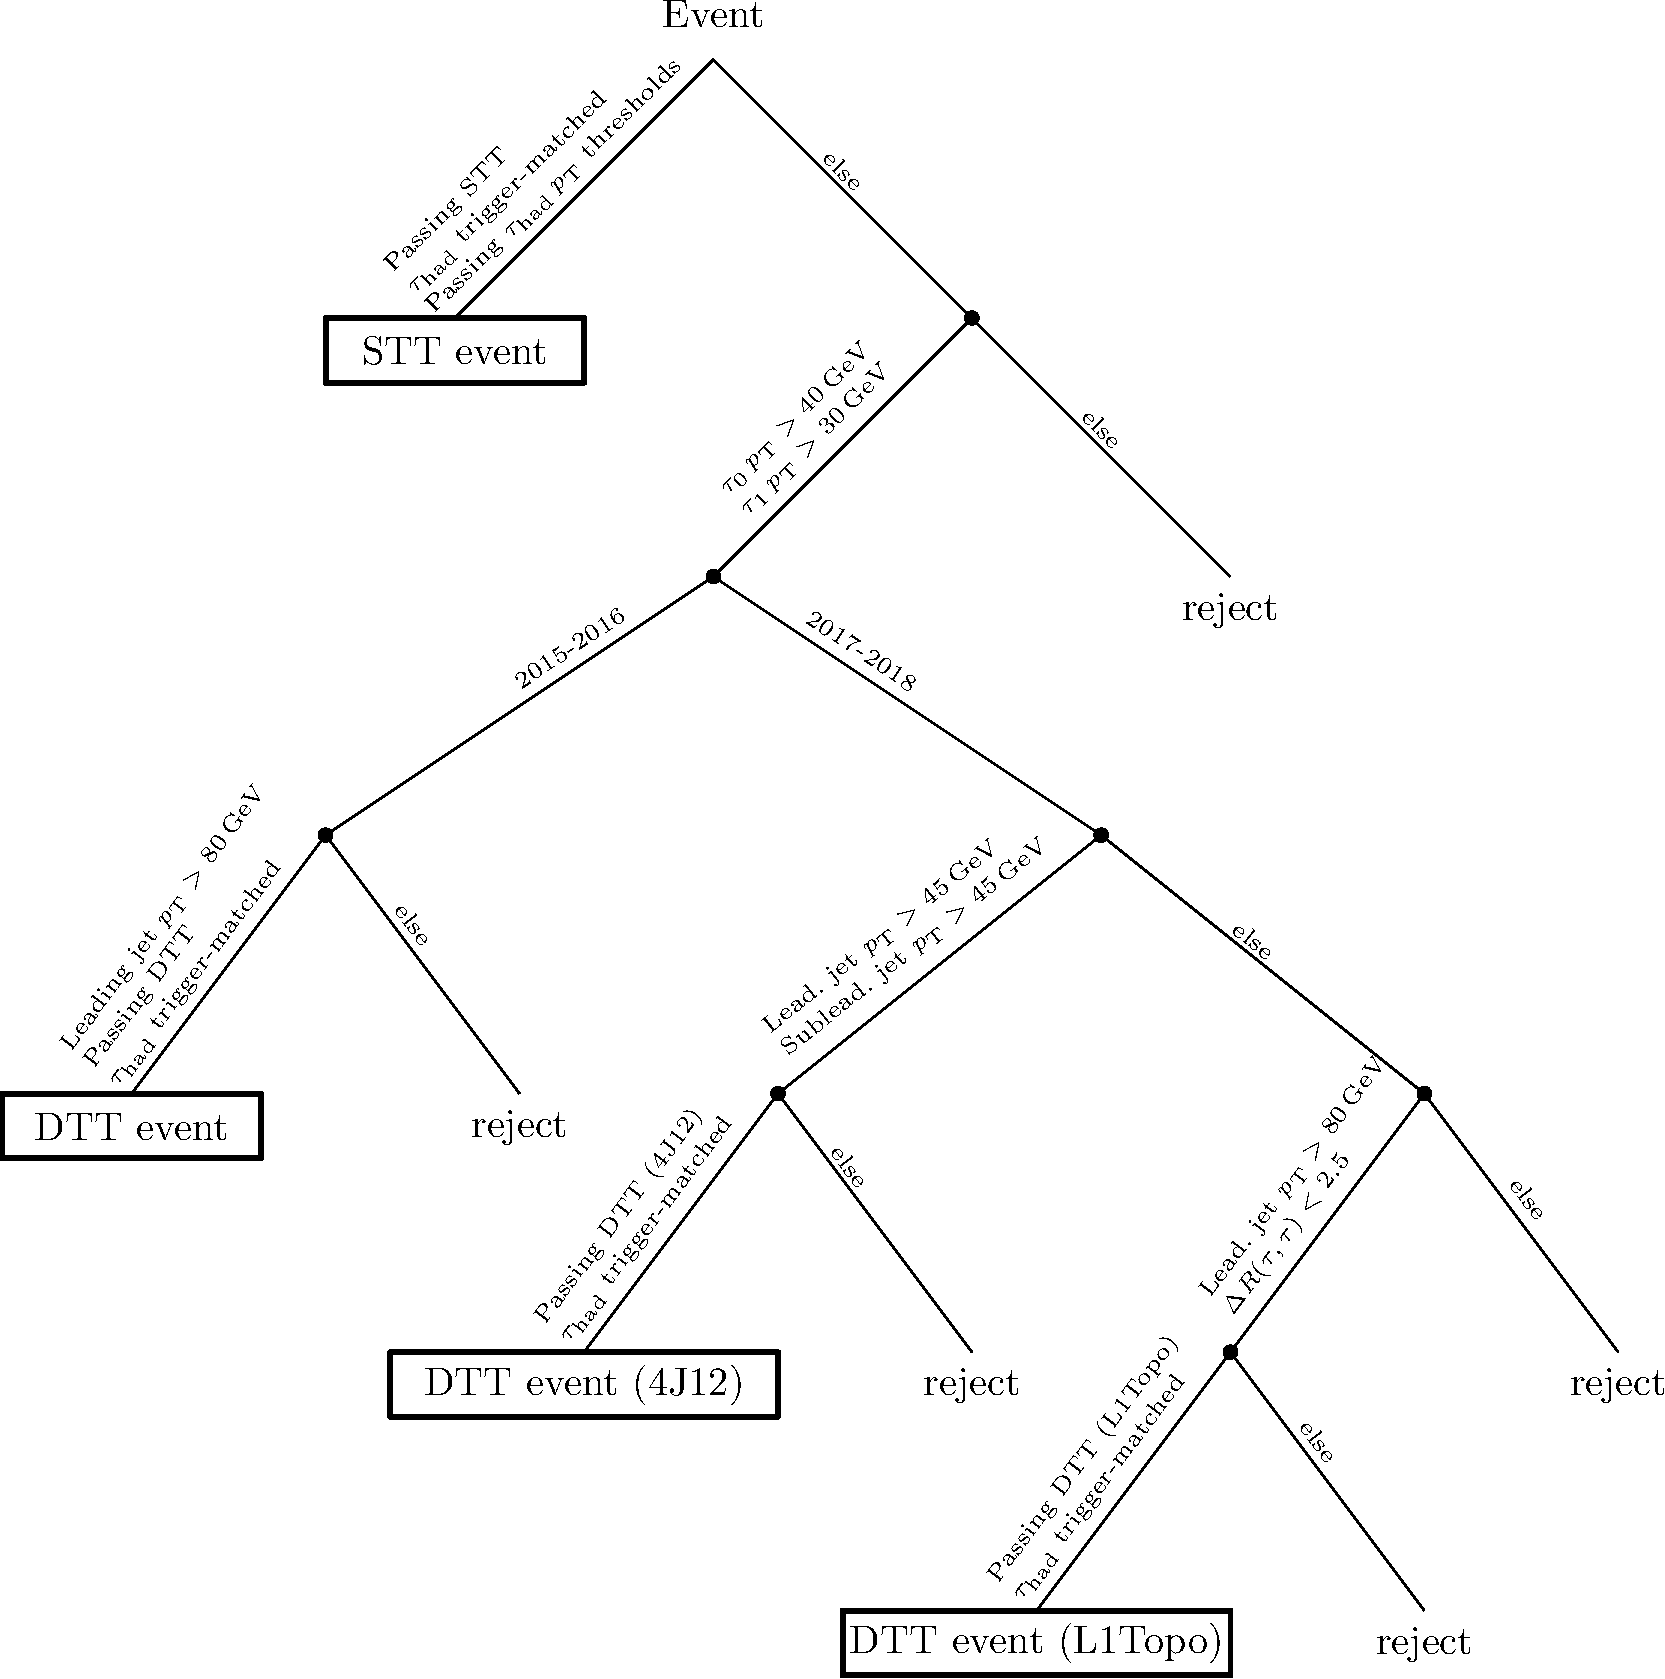
\includegraphics[width=0.8\textwidth]{figures/selection/HadHad_HH/trigger_flowchart_hadhad}
  \caption{Flowchart of the $\tauhad\tauhad$ trigger selection. ``Pass
    STT / DTT'' refers to checking whether the trigger selected the
    event (cf.~\Cref{tab:triggers_hadhad} for the triggers relevant
    for each run period).}
  \label{fig:hadhad_trigger_flowchart}
\end{figure}

A small inconsistency is present in the separation of the STT and DTT
trigger channels (c.f.\ first branching
in~\Cref{fig:hadhad_trigger_flowchart}). This is illustrated in the
following starting with the correct method that is used for the
sub-categorization of DTT events.

The categorization of DTT events is performed by first checking the
offline thresholds corresponding to the trigger of interest. Only if
these thresholds are fulfilled it is checked whether the trigger
selected the event and the reconstructed \tauhad are geometrically
matched to the HLT objects. If the offline thresholds are fulfilled
but the trigger did not select the event or the trigger-matching
failed, the event is rejected and not considered for any other
trigger-channel.

When distinguishing between STT and DTT categories this is not done
purely using offline reconstructed quantities since it is
simultaneously checked whether the event passes offline thresholds and
trigger-matching. This means that events that pass STT offline
thresholds but fail STT trigger-matching are still considered as
candidates in the DTT category (unlike the correct approach that is
used for DTT event sub-classification where these events are rejected
and not considered for further categorization). This would be
problematic when applying \tauhad trigger calibrations in the DTT
channel because there can be events that were explicitly checked to
fail STT-matching which violates the assumptions of the \tauhad
trigger calibration measurement. The fraction of events that pass the
STT thresholds but were not selected by the STT was checked and it was
found that only 0.1 to 0.2\,\% of events in the signal region are
affected. Therefore, this inconsistency has negligible effect on the
analysis.

More studies motivating the choices regarding the trigger strategy in
$bb\hadhad$ can be found in~\Cref{subsec:hadhad_trigger_studies}.
